
    \begin{frame}{Implicit Processes}
        \textbf{\alert{Motivation}}: Gaussian processes are limited by the parametric kernel family.

        \begin{itemize}
            \item Square exponential kernel: \(\kappa(\mathbf x_1, \mathbf x_2) = \sigma^2 \exp \left(- \frac{\|\mathbf x_1 - \mathbf x_2 \|_2^2}{2l^2} \right) \).
            \item Linear kernel: \(\kappa(\mathbf x_1, \mathbf x_2) = a \mathbf x_1^T \mathbf x_2 + b\).
        \end{itemize}

        \begin{figure}
            \centering
            \begin{tabular}{cc}
              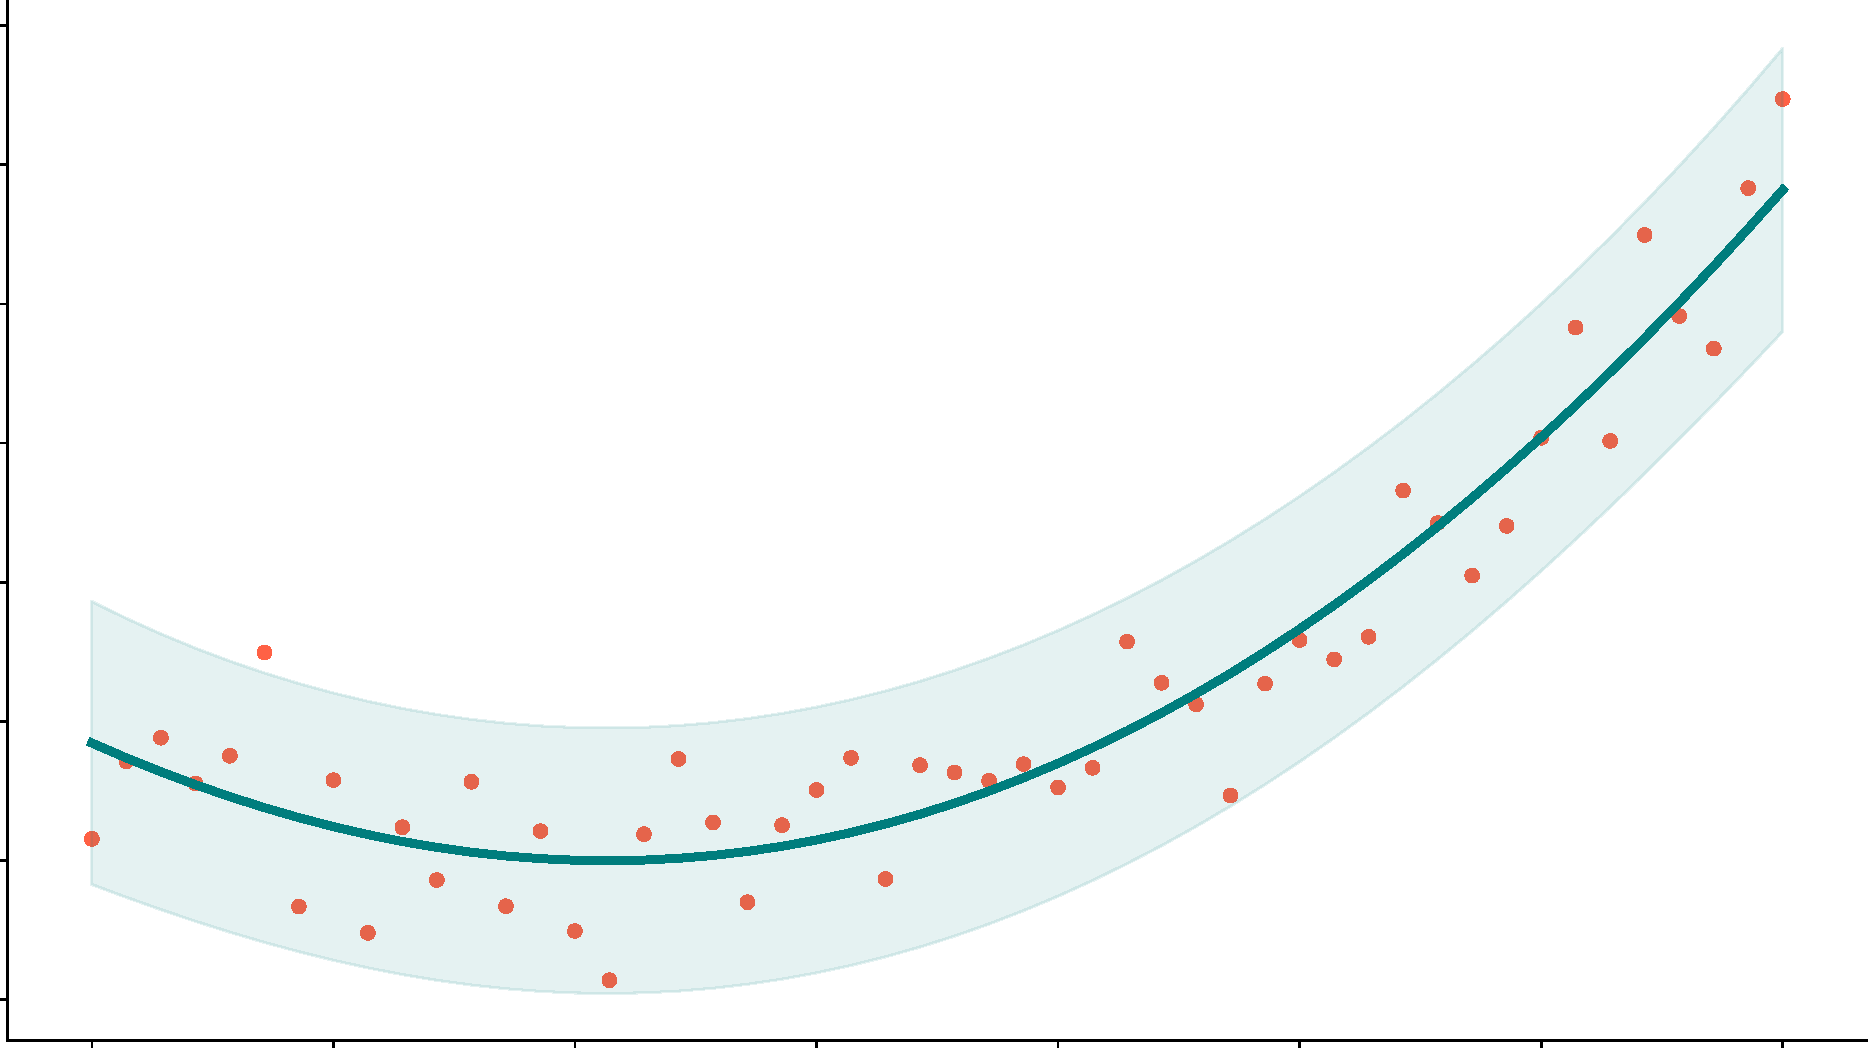
\includegraphics[width=.46\linewidth]{imgs/GP_RBF.pdf} &
              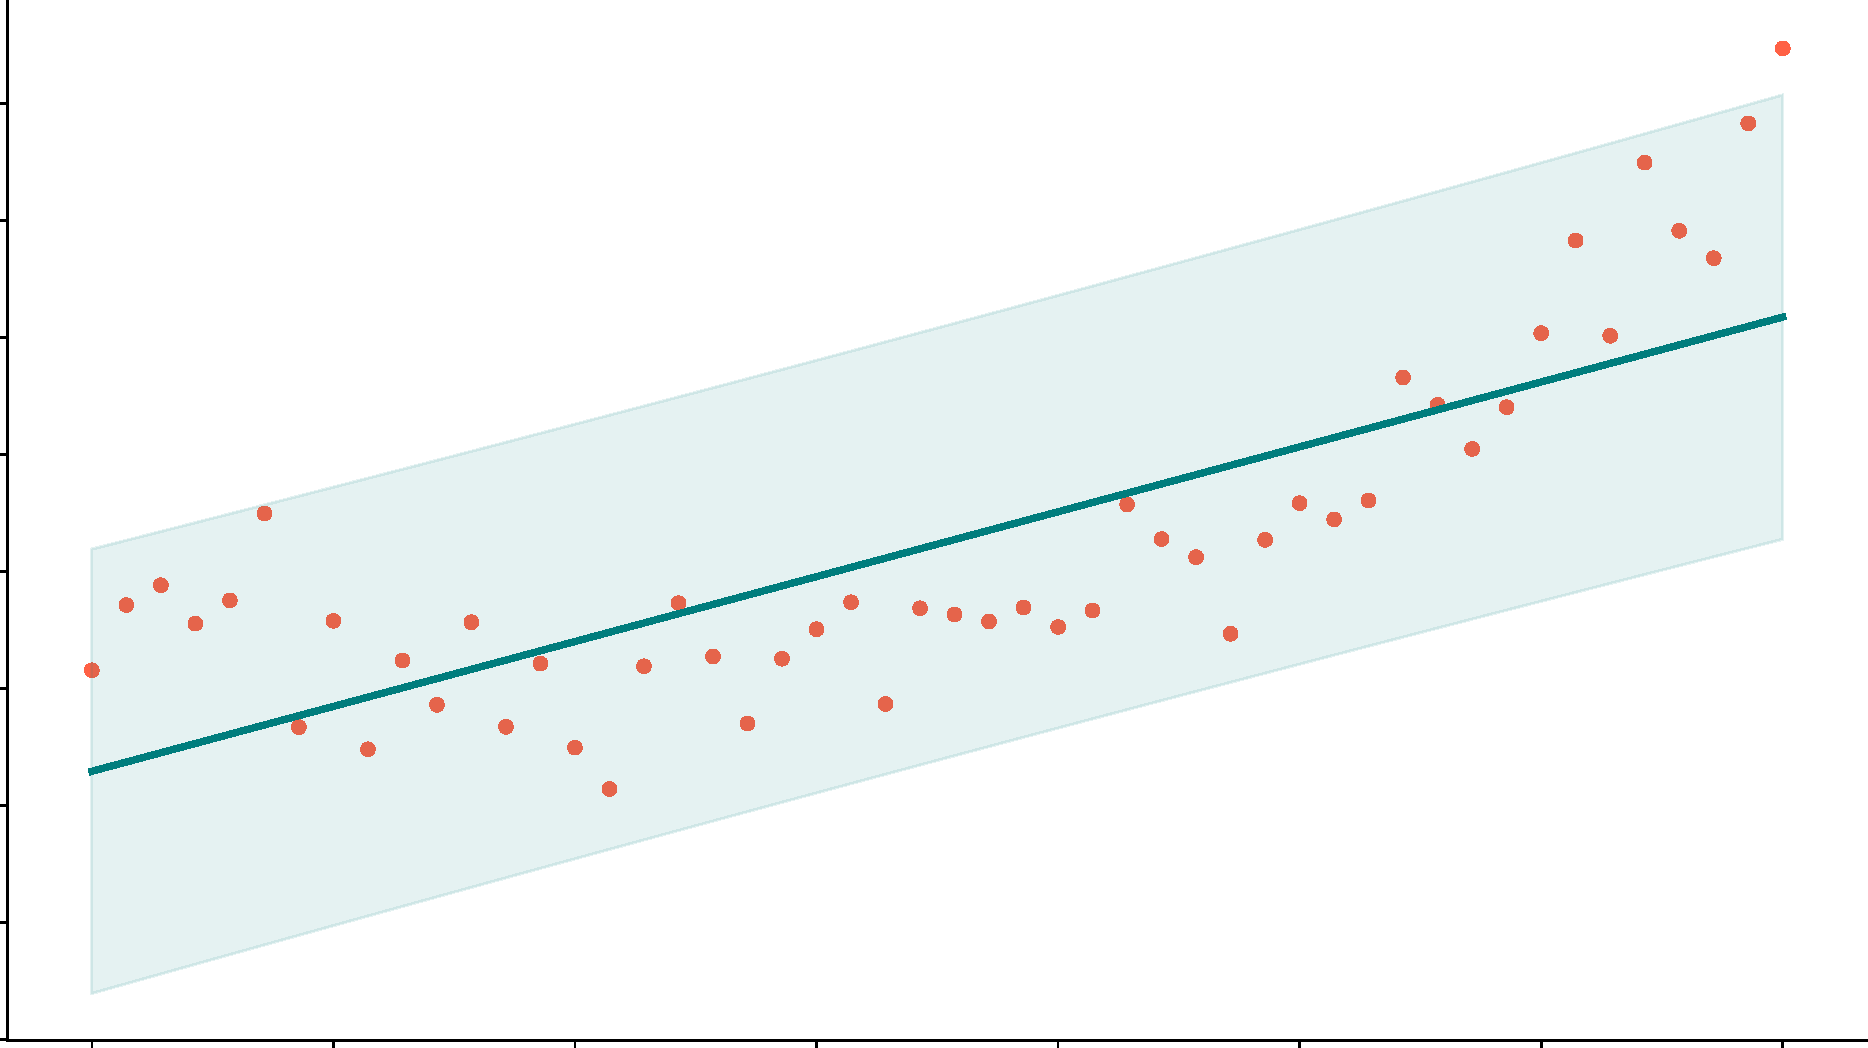
\includegraphics[width=.46\linewidth]{imgs/GP_DOT.pdf}
            \end{tabular}
        \end{figure}
        The Gaussian process prior over functions is \textbf{\alert{too restrictive}}.
    \end{frame}

    \begin{frame}
    \begin{overprint}
        An \textbf{\alert{implicit stochastic process}}\footnote{
Ma, C., Li, Y. \& Hernandez-Lobato, J.M.. (2019). Variational Implicit Processes.} (IP) is a collection of random variables \( f(\cdot) \) such that any finite collection \( \mathbf f = \{f(\mathbf x_1), f(\mathbf x_2), \dots, f(\mathbf x_N) \} \) is implicitly defined by the following generative process:
        \[
            \mathbf z \sim P_{\mathbf z}(\mathbf z) \quad \text{\emph{and}} \quad f(\mathbf x_n) = g_{\mathbf \theta}(\mathbf x_n, \mathbf z), \ \forall n =1, \dots, N\,.
        \]
        \end{overprint}
    \begin{overprint}
    \onslide*<2>{
        \textbf{Gaussian process}
            \[
                \mathbf z \sim \mathcal{N}(\bm 0, \bm I) \quad \text{\emph{and}} \quad f(\mathbf x_n) = \bm L(\mathbf x_n)^T\mathbf z, \ \forall n =1, \dots, N\,.
            \]
    }
    \onslide*<3>{
        \begin{minipage}{0.4\textwidth}
            \textbf{Bayesian Neural Networks}. 
            \[
                (\mathbf z_1, \mathbf z_2) \sim \mathcal{N}(\bm 0, \bm I)
            \]
            \[
                \bm \theta = (\bm \mu_1, \bm \mu_2, \bm \sigma_1, \bm \sigma_2)
            \]
            \[
                \bm h = r((\bm \mu_1 + \bm \sigma_1 \mathbf z_1)^T\mathbf{x}_n)\,.
            \]
            \[
                g_{\mathbf \theta}(\mathbf x_n, \mathbf z) = (\bm \mu_2 + \bm \sigma_2 \mathbf z_2)^T \bm h
            \]
        \end{minipage}%
        \begin{minipage}{0.6\textwidth}
        \begin{figure}
            \centering
            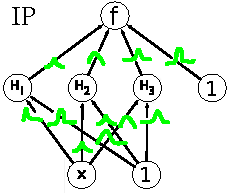
\includegraphics[width=0.6\textwidth]{imgs/BNN.pdf}
        \end{figure}
        \end{minipage}
    }
    \end{overprint}
    \end{frame}



    \begin{frame}{Variational Inference on Implicit Processes}
    \textbf{Problem statement:}
        \begin{enumerate}
            \item The unknown target function \textbf{is a sample from an IP}, that is, an implicit distribution over stochastic processes \(P(f(\cdot))\).
            \item Given the set of observations \((\mathbf X, \mathbf y)\), we aim to approximate the posterior distribution over functions \(P(f(\cdot)| \mathbf X, \mathbf y)\).
        \end{enumerate}
        \textbf{Approach}: Use variational inference over the function-space distribution \(Q(f(\cdot))\).
        \[
        \begin{aligned}
        Q^\star(f(\cdot))&= \argmin_{Q \in \mathcal{Q}}\, KL\Big(Q(f(\cdot))  \mid P( f(\cdot) | \mathbf X, \mathbf y)\Big)\\
        &= \argmax_{Q \in \mathcal{Q}} \,\mathbb{E}_{Q(f)}\Big[ \log P(\mathbf y | \mathbf X, f(\mathbf X)) \Big] - KL\Big(Q(f(\cdot)) \mid P(f(\cdot)) \Big)\,.
        \end{aligned}
        \]
    \end{frame}
    \begin{frame}
        \textbf{Approach}: Use variational inference over the function-space distribution
        \[
            Q^\star(f(\cdot)) = \argmax_{Q \in \mathcal{Q}} \,\mathbb{E}_{Q(f)}\Big[ \log P(\mathbf y | \mathbf X, f(\mathbf X)) \Big] - KL\Big(Q(f(\cdot)) \mid P(f(\cdot)) \Big)\,.
        \]
        \textbf{Difficulties:}
        \begin{enumerate}
            \item The prior \(P(f(\cdot))\) lacks a closed form.
            \item The Kullback-Leibler divergence between stochastic processes is not well-defined.
            \item The variational distribution \(Q(f(\cdot))\) must allow to compute or approximate by samples the data-fitting term.
        \end{enumerate}
    \end{frame}

    \begin{frame}{Existing Approaches}
        \textbf{\alert{Variational Implicit Processes}}\footnote{
            Ma, C., Li, Y. \& Hernandez-Lobato, J.M.. (2019). Variational Implicit Processes.}: Approximates the distribution over functions using a \textbf{linear combination of samples}.\\
        \vspace{0.5cm}
        \textbf{\alert{Sparse Implicit Processes}}\footnote{
            Rodríguez-Santana, S., Zaldivar, B. \& Hernandez-Lobato, D.. (2022). Function-space Inference with Sparse Implicit Processes.}: Uses \textbf{inducing points} for scalability and approximates the KL using an \textbf{external discriminator} (a Neural Network).\\
        \vspace{0.5cm}
        \textbf{\alert{Linearized approximation}}\footnote{
            Rudner, T., Chen, Z., Whye Y. \& Gal, Y.. (2022). Tractable Function-Space Variational Inference in Bayesian Neural Networks.}: Approximates the distribution over functions using a \textbf{linearization} of the BNN over the parameters.
    \end{frame}

    \subsection{Variational Implicit Processes}
    \begin{frame}{Variational Implicit Processes}
        Approximate \(P(f(\cdot))\) with a GP \(P_{\mathcal{GP}}(f(\cdot))\) \textbf{based on samples} \(f_1(\cdot),\dots,f_S(\cdot)\).
        Let
        \[
            \hat{m}(\mathbf x) = \frac{1}{S}\sum_{s=1}^S f_s(\mathbf x), \quad            \hat{\mathbf \phi}(\mathbf x) = \frac{1}{\sqrt{S}}  \Big(f_1(\mathbf x) - \hat{m}(\mathbf x), \ldots, f_S(\mathbf x) - \hat{m}(\mathbf x)\Big)^T\,.
        \]
        Then, setting a standard \textbf{Gaussian prior} \(P(\mathbf a) = \mathcal{N}(\mathbf a | \mathbf 0, \mathbf I)\),
        \[
            \hat{f}(\mathbf x) = \hat{m}(\mathbf x) + \mathbf a^T \hat{\mathbf \phi}(\mathbf x) \implies P_{\mathcal{GP}}(\hat{f}(\mathbf x)) = \mathcal{N}(\hat{m}(\mathbf x), \hat{\mathbf \phi}(\mathbf x)^T\hat{\mathbf \phi}(\mathbf x))\,.
        \]

        Using a variational distribution \(Q(\mathbf a) = \mathcal{N}(\mathbf m, \mathbf S)\) induces a variational distribution over functions
        \[
            Q(\hat{f}(\mathbf x)) = \int_{\bm a}P(\hat{f}(\mathbf x) | \bm a)Q(\bm a) = \mathcal{N}\Big(\hat{m}(\mathbf x) + \,\hat{\mathbf \phi}(\mathbf x)^T\mathbf m, \hat{\mathbf \phi}(\mathbf x)^T\mathbf S\hat{\mathbf \phi}(\mathbf x)\Big)\,.
        \]

    \end{frame}
    \begin{frame}
        Naming
        \[
        \hat{\mathbf{f}} = (\hat{f}(\mathbf x_1),\dots, \hat{f}(\mathbf x_N))\,.
        \]
        The ELBO is computed to minimized the KL divergence evaluated on \(\hat{\mathbf{f}}\) and \(\bm a\) rather than between stochastic processes
        \[
        \begin{aligned}
            &\cancel{Q^\star(f(\cdot)) = \argmin_{Q \in \mathcal{Q}}\, KL\Big(Q(f(\cdot))  \mid P( f(\cdot) | \mathbf X, \mathbf y)\Big)}\\
            &Q^\star (\hat{\mathbf{f}}, \bm a) = \argmin_{Q \in \mathcal{Q}}\, KL\Big(Q(\hat{\mathbf{f}}, \bm a)  \mid P( \hat{\mathbf{f}}, \bm a | \mathbf X, \mathbf y)\Big)\\
            &\hspace{0.9cm} = \argmax_{Q \in \mathcal{Q}} \,\mathbb{E}_{Q(\hat{\mathbf{f}})}\Big[ \log P(\mathbf y | \mathbf X, \hat{\mathbf{f}}) \Big] - KL\Big(Q(\bm a) \mid P(\bm a) \Big)\,.
        \end{aligned}
        \]

    \end{frame}
    
    \subsection{Sparse Implicit Processes}
    \begin{frame}{Sparse Implicit Processes}
        \begin{enumerate}
            \item Considers an \textbf{inducing points} approach, leading to the ELBO
                \[
                    \mathcal{L} = \mathbb{E}_{Q(\mathbf{f})}\Big[ \log P(\mathbf y | \mathbf X, \mathbf{f}) \Big] - KL\Big(Q(\bm u) \mid P(\bm u) \Big)\,.
                \]
            \item The variational distribution of the inducing points \(Q(\bm u)\) is an \textbf{IP}.
            \item The Kullback-Leibler term is approximated using an \textbf{external discriminator} \(T\) (a neural network),
            \[ 
             KL\Big(Q(\bm u) \mid P(\bm u) \Big) \approx \mathbb{E}_{Q(\bm u)}[T(\bm u)]\,.
            \]
            \item The data-fitting term is \textbf{approximated using Monte-Carlo} samples of \(Q(\bm u)\),
            \[
                Q(\mathbf f) = \int_{\bm u}P(\mathbf f |\bm u)Q(\bm u) \approx \frac{1}{S} \sum_{s=1}^S P(\mathbf f | \bm u_s)\,,
            \]
            where \(P(\mathbf f | \bm u)\) is approximated as Gaussian with mean and covariances estimated empirically from the prior.
        \end{enumerate}
        
    \end{frame}

    \subsection{Linearized approximation}
    \begin{frame}{Linearized approximation}
        Seeing the stochastic function \(f(\cdot, \bm \theta)\) defined in terms of the stochastic parameters \(\bm \theta\) according to a distribution \(P_{\bm \Theta}\), with 
        \[
        P_{\bm \Theta} = \mathcal{N}(\bm m, \bm S)\,.
        \]
        The stochastic function can be approximated with a \textbf{Taylor approximation of order 1 over the parameter space, centered on \(\bm m\),}
        \[
            f(\cdot, \bm \theta) \approx \hat{f}(\cdot, \bm \theta) = f(\cdot, \bm m) + \mathcal{J}(\cdot, \bm m)(\bm \theta - \bm m)\,,
        \]
        where 
        \[
            \mathcal{J}(\cdot, \bm m) = \frac{\partial f(\cdot, \bm \theta)}{\partial \bm \theta}(\bm m)\,.
        \]
        As a result, \(\hat{f}(\cdot, \bm \theta)\) is a \textbf{\alert{Gaussian process}},
        \[
             \hat{P}(\hat{f}(\cdot, \bm \theta)) = \mathcal{N}(f(\cdot, \bm m), \mathcal{J}(\cdot, \bm m) \bm S \mathcal{J}(\cdot, \bm m)^T)\,.
        \]    
    \end{frame}

    \begin{frame}

        \[
        \mathcal{L} = \mathbb{E}_{Q(f))}\Big[ \log P(\mathbf y | \mathbf X, f(\mathbf X)) \Big] - KL\Big(Q(f(\cdot)) \mid P(f(\cdot)) \Big)
        \]
    
        Using a variational distribution over the parameters \(Q_{\bm \Theta}\), \textbf{leads to a variational distribution over the stochastic functions} \(Q(f)\), where samples can be easily taken.

        The Kullback-Leibler divergence between stochastic processes can be defined using evaluations
        \[
            KL\Big(Q(f(\cdot)) \mid P(f(\cdot)) \Big) = \sup_{\mathbf C \in 2^\mathcal{X}} KL\Big(Q(f(\mathbf C)) \mid P(f(\mathbf C)) \Big)\,.
        \]
        Therefore, \textbf{approximated empirically} using the linearized models on a set of \textbf{Context points} \(\{\mathbf C_1, \dots, \mathbf C_S\}\),
        \[
            KL\Big(Q(f(\cdot)) \mid P(f(\cdot)) \Big) \approx \max_{\mathbf C \in \{\mathbf C_1, \dots, \mathbf C_S\}} KL\Big(\hat{Q}(\hat{f}(\mathbf C)) \mid \hat{P}(\hat{f}(\mathbf C)) \Big)\,,
        \]
        which is a KL between Gaussian distributions.
    \end{frame}
    
    \begin{frame}{Limitations}
    \begin{itemize}
        \item \textbf{Variational implicit processes}. The linear approximation can be too strong,
        \[ 
            f(\mathbf x) \approx \hat{m}(\mathbf x) + \bm a^T \hat{\phi}(\mathbf x)\,.
        \]
        \item \textbf{Sparse Implicit Processes}. Relies on an external discriminator \(T\), increasing the training time due to a double-loop training.
        \[ 
             KL\Big(Q(\bm u) \mid P(\bm u) \Big) \approx \mathbb{E}_{Q(\bm u)}[T(\bm u)]\,.
        \]
        \item \textbf{Linearized approximation}. The set of \textbf{Context points} \(\{\mathbf C_1, \dots, \mathbf C_S\}\) must be defined by hand previously to any learning. With points both \textbf{in the training space and out of the training space} to ensure generalization.
        \[
            KL\Big(Q(f(\cdot)) \mid P(f(\cdot)) \Big) \approx \max_{\mathbf C \in \{\mathbf C_1, \dots, \mathbf C_S\}} KL\Big(\hat{Q}(\hat{f}(\mathbf C)) \mid \hat{P}(\hat{f}(\mathbf C) )\Big)\,.
        \]
    \end{itemize}
    \end{frame}